%deixar chapter vazio - exatamente como está. Preencher o documento apenaas apartir de section.
\chapter*[]{}

\section{Tema}

Simulação Computacional.

\subsection{Delimitação do tema}

Detecção de colisão entre objetos em simulações computacionais.

\section{Problema}

 Estudar e avaliar os mecanismos para detecção de colisão em uma simulação computacional que busca apresentar objetos de forma mais realística possível.


\section{Objetivos}
\subsection{Objetivo Geral}
Explicar como funciona a detecção de colisão em simulações computacionais.

\subsection{Objetivos Específicos}
\begin{enumerate}
\item Conhecer as principais etapas de uma simulação física computacional.
\item Avaliar o funcionamento dos algoritmos sort and sweep e octree na fase de detecção de possíveis colisões em uma etapa de simulação.
\item Avaliar o funcionamento de algoritmos para detecção de colisão entre objetos de geometrias específicas.
\item Avaliar o método Impulse para a resolução de colisão entre dois objetos em uma etapa de simulação.
\end{enumerate}

\section{Justificativa}

Segundo \citeonline{bourg2013physics}, “a detecção de colisão é um problema de geometria computacional que determina se ocorreu, e onde ocorreu, uma ou mais colisões entre objetos” da simulação. Com base nisto, podemos afirmar que existem diversos algoritmos para detecção de colisão entre objetos de geometrias específicas, e também diferentes técnicas para otimizar esta detecção tornando-a mais eficiente, rápida e robusta.

\citeonline{ericson2004real} afirma que apesar de hoje em dia os computadores serem extremamente rápidos, a detecção de colisão continua sendo um problema fundamental. Isso ocorre porque jogos e outras simulações são frequentemente construídos em um ambiente 3D, com centenas de milhares de polígonos, exigindo assim, algoritmos e estruturas de dados mais sofisticados para operar, em tempo real, com conjuntos de dados dessa magnitude.

Por ser uma área ainda em expansão, pouco explorada e conhecida, este estudo se justifica pois novos métodos poderão surgir, havendo possibilidades para vários trabalhos de pesquisa e desenvolvimento.

\section{Referencial Teórico}

Nesta sessão, é apresentada o estudo teórico sobre os principais tópicos envolvendo a detecção de colisão em ambientes simulados.

\subsection{Simulação Computacional}

Segundo \citeonline{duran2018computer} A simulação computacional é uma técnica amplamente utilizada para o estudo de
sistemas complexos que por diversos fatores não podem ser facilmente
reproduzidos devido a custos elevados, ou pelo tempo necessário para que se
realize os experimentos para a obtenção de resultados precisos.

A simulação permite que um pesquisador avalie diversos cenários diferentes para sua
pesquisa apenas alterando suas variáveis de controle reduzindo a sim os custos
e os riscos de um experimento físico. Essa técnica pode ser aplicada em
diversas áreas como biologia, engenharia, física, química entre outras.

Para construir uma simulação, torna-se necessária a representação matemática ou
computacional do comportamento do sistema a ser simulado. Isso inclue mas não
se limita a variáveis de controle que podem alterar o ambiente simulado, e os
objetos que serão simulados durante algumas etapas, ou por um período de tempo.

A simulação é uma poderosa ferramenta que contribue na descoberta de novas
tecnologias, ou no aprimoramento das existentes.


\subsubsection{Representação Computacional de Formas Geométricas}
Na computação, não existe maneira correta ou incorreta de representar a
geometria. A forma usada dependerá  do nível de detalhamento desejado. É possível fazer esta representação de diversas maneiras, por exemplo: forma vetorial, paramétrica ou de forma poligonal.

Neste estudo será adotada a representação vetorial, devido a sua simplicidade e fácil compreensão. O trabalho será desenvolvido com 3 geometrias principais, que são: esferas, caixas e poliedros.

Para representação dessas formas geométricas, são utilizados pontos de coordenadas cartesianas, definidos em uma estrutura de vetor tridimensional. demonstrado no Código~\ref{code:vec_1}

\begin{lstlisting}[frame=single,caption=Exemplo de vetor 3d\label{code:vec3d_1}]
class vector3d{
float x;
float y;
float z;

vector3d(float x, float y, float z){
this->x=x;
this->y=y;
this->z=z;
}
};
\end{lstlisting}

Onde x representa o eixo que vai da esquerda para a direita;
y representa o eixo  perpendicular ao eixo x;
e z é o eixo que indica a profundidade apontando para cima.


Lembrando também que os vetores tem diversas operações relacionadas como soma,
subtração, multiplicação, divisão, comprimento ou módulo, produto escalar,
produto cruzado e produto triplo escalar que são relevantes para este estudo.

\subsubsection{Esferas}

As esferas são simples de representar computacionalmente, e também
incrivelmente fáceis de se computar. Para representarmos uma esfera, tudo o que
precisamos é de um ponto que representará o centro da esfera, e um raio, que
indica o quanto a esfera se estende em todas as direções a partir do centro.
Em \citeonline{ericson2004real} é possível encontrar uma implementação geral de esferas, e em \citeonline{bourg2013physics} é possível perceber na prática como usar uma bounding sphere.

\begin{lstlisting}[frame=single,caption=Representação de esfera\label{code:sphere3d}]
class sphere3d {
public:
vector3d center;
float radius;
sphere3d(const vector3d& center, float radius)
{
this->center=center;
this->radius=radius;
}
};

sphere3d s({0.0f, 0.0f, 0.0f}, 5.0f);
\end{lstlisting}

Desta forma, temos uma esfera cujo o centro está posicionado exatamente na origem de
nosso sistema cartesiano, e que se estende por um raio de 5 em todas as
direções.

\subsubsection{Caixas}

As caixas são trivialmente representáveis de diversas formas. Com elas podemos
representar formas cuboides facilmente. Ela normalmente é representada por dois
vetores, onde um indica o canto inferior esquerdo, e o outro o canto superior direito.

Outras formas populares de se representar caixas são:
Ponto central mais meias larguras que se estenderão do centro até as bordas da caixa.
Ponto inferior esquerdo, e a extensão de suas arestas no eixo x, y e z.
As três formas apresentadas no Código~\ref{code:box3d_1}, ~\ref{code:box3d_2} e ~\ref{code:box3d_3} fornecem vantagens e
desvantagens dependendo do contexto em que forem utilizadas.
Em \citeonline{ericson2004real} é possível encontrar uma explicação mais detalhada de como estas representações funcionam.

Caixa representada pelo ponto mínimo e máximo:

\begin{lstlisting}[frame=single,caption=Representação de caixa ponto mínimo e máximo\label{code:box3d_1}]
class box3d_1{
vector3d min;
vector3d max;
};
\end{lstlisting}

Caixa com meia larguras

\begin{lstlisting}[frame=single,caption=Exemplo de caixa com meias larguras\label{code:box3d_2}]
class box3d_2
{
vector3d center;
vector3d radius;
};
\end{lstlisting}

Caixa com ponto mínimo e medidas completas:

\begin{lstlisting}[frame=single,caption=Exemplo de caixa  com arestas\label{code:box3d_3}]
class box3d_3 {
vector3d min;
vector3d measures;
};
\end{lstlisting}

Todas elas servem para representar a mesma coisa, mas podem ser utilizadas em
contextos diferentes dependendo o requisito. O Código~\ref{code:box3d_1} é excelente para aabbs
porque já tem seus limites bem definidos e pode ser usada mais facilmente para
sucessivos testes. Porém tem a desvantagem de precisar fazer uma atualização
extra quando precisar ser movimentada.

No entanto, o Código~\ref{code:box3d_2} tem a vantagem de precisar atualizar apenas o ponto
central, porém, quando necessário, terá as operações para computar seus pontos
mínimos e máximos. Este tipo de estrutura também é conhecida como esfera de 3
raios.

Em octrees ela é a representação preferida para a representação de nós
pois é fácil de representar e de se computar.

O Código~\ref{code:box3d_3} Lembra muito a criação de uma janela na computação gráfica. Ela tem seu
ponto mínimo, e o comprimento de suas arestas até o ponto máximo.

O Código~\ref{example_box3d} cria três caixas exatamente iguais.

\begin{lstlisting}[frame=single,caption=Código de exemplo de criação de 3 caixas\label{example_box3d}]
box3d_1 b1({10,10,10}, {20,20,20});
box3d_2 b2({15,15,15}, {5,5,5});
box3d_3 b3({10,10,10}, {10,10,10});
\end{lstlisting}

Todas as 3 representações terão seus limites entre 10 e 20.


\subsubsection{Poliedros}

Os poliedros nada mais são que uma nuvem de pontos que representam uma
geometria específica. Os poliedros certamente são a maneira mais precisa de
representar geometria, porém eles apresentam uma dualidade significativa. Quanto mais
detalhado o poliedro, mais caro será para computar colisões, rotações e
translações.

Existem dois tipos de poliedros. Poliedros convexos e poliedros
côncavos. Poliedros convexos são poliedros que são coplanares ou que possuem
suas faces voltadas para fora. Por outro lado, poliedros côncavos possuem
pelo menos uma de suas faces voltada para o interior.
Neste trabalho não usaremos poliedros pois eles utilizam algoritmos mais
sofisticados para operarem sobre nuvens de pontos para detectar colisões.
Em \citeonline{ericson2004real} é discutido com mais detalhes poliedros e seus algoritmos específicos.

\subsection{ Estruturas para delimitação de volumes}

Em uma simulação computacional existem diversos objetos e o ambiente precisa testar se alguma colisão ocorreu. Este monitoramento constante acaba tendo um alto custo computacional. Para otimizar esse processo, os simuladores utilizam estruturas chamadas delimitadores de volume, que fazem um encapsulamento da geometria em avaliação.

Existem vários tipos de estruturas delimitadoras de volumes, como esferas, retângulos, e cascas convexas. Devido a simplicidade de implementação, neste trabalho optou-se pela estrutura retangular. As estruturas delimitadoras de volume poderão ser implementadas de duas formas básicas, que são: Aligned Axis Bounding Box (AABB) e Oriented Bounding Box (OBB).

A estrutura AABB, que pode ser implementada como apresentado no Código~\ref{code:aabb_1}, é uma caixa retangular alinhada aos três eixos do sistema de coordenadas e não pode sofrer rotações. Caso uma rotação aconteça, o delimitador precisa ser reconstruído, implicando em maior custo computacional. No entanto, segundo \citeonline{ericson2004real}, a verificação de colisão é relativamente mais simples de computar.

\begin{lstlisting}[frame=single,caption=Exemplo de AABB\label{code:aabb_1}]
class AABB
{
public:
vector3d min;
vector3d max;
GeometricShape* shape;
};
\end{lstlisting}

\begin{lstlisting}[frame=single,caption=Exemplo de AABB e Esfera\label{code:aabbSphere}]
sphere3d* s=new sphere3d({5, 5, 5}, 5);
AABB* aabb=new AABB(s);
\end{lstlisting}


Como apresentado no Código~\ref{code:aabbSphere}, a bounding box desta esfera será 2 vetores encapsulando completamente em um cubo. Seus vetores respectivamente serão: min=0,0,0 max=10,10,10

Já a estrutura OBB não está presa a nenhum eixo, facilitando a rotação dos objetos contidos nela. A estrutura OBB, apresentada no Código~\ref{code:obb_1},  é representada por um ponto central, com meias medidas para os eixos e uma matriz de rotação. Segundo Ericson a estrutura OBBS é computacionalmente custosa e de difícil implementação.

\begin{lstlisting}[frame=single,caption=Código de exemplo de OBB\label{code:obb_1}]
class obb
{
public:
vector3d center;
vector3d measures;
matrix3x3 orientation;
};
\end{lstlisting}

Neste trabalho optou-se pela utilização da estrutura AABB, devido à relativa facilidade de implementação em relação a estrutura OBB

\subsubsection{Corpo Rígido}
Segundo \citeonline{bourg2013physics} Um corpo rígido é um conjunto de partículas  que permanecem a distâncias fixas umas das outras  sem nenhum tipo de translação ou rotação entre elas. Em outras palavras,  um corpo rígido não mudará de forma enquanto se move, ou sua deformação é tão insignificante que pode ser desprezada.

Um corpo rígido é  frequentemente representado como tendo uma posição, uma orientação  e  dimensões para representar seu volume. Estes são requisitos mínimos para a  sua definição, porém, dependendo do nível de precisão desejada, pode-se adicionar mais atributos como tensores de inércia, velocidades lineares e angulares, coeficiente de restituição, e o que mais for necessário para que se atinja os objetivos desejados.

Existem 3 classes principais de corpos que podem ser representadas em uma simulação:
Corpos rígidos, que não se deformam  enquanto se movem, ou caso se deformem, são capazes de voltar a sua forma original;


Corpos macios, que podem deformar enquanto se movem ou por ação de forças ou eventos externos;

Ou corpos estáticos, que nada mais é que uma sub-classificação de um corpo rígido ou um corpo macio,  mas com a ausência de massa, ficando a sim, estacionário na posição em que se
encontra...

\subsubsection{Representação de um Corpo Rígido}

Para fins de exemplos, a seguinte representação de corpo rígido será adotada:

\begin{lstlisting}[frame=single,caption=Exemplo de corpo rígido\label{code:RigidBody}]
class RigidBody
{
public:
float mass;
float restitution;
vector3d lastPosition;
vector3d position;
vector3d velocity;
vector3d forces;
AABB* aabb;
};
\end{lstlisting}

\subsection{Detecção de Colisão}
Segundo \citeonline{bourg2013physics}, a detecção de colisão é um problema de geometria computacional que
determina se e onde, dois ou mais objetos colidiram.
Uma colisão pode ser detectada de diversas maneiras dependendo da natureza dos
objetos envolvidos como esferas e caixas.

Para algumas situações, uma colisão pode ser detectada se a distância entre os dois objetos está abaixo de uma
determinada tolerância. Em outros casos, os objetos podem estar se sobrepondo
em um ou mais pontos.

Após uma colisão ser detectada, diversos dados precisam ser coletados para o processamento e resolução da colisão, que é feito posteriormente. Os dados coletados dependerão da natureza do simulador. Para um simulador de física, por exemplo, pode ser necessário o ponto ou pontos de contato onde os objetos colidiram, bem como a velocidade relativa destes objetos no instante da colisão.

Outros dados relevantes para coleta na detecção de colisão são: o vetor normal, que é um vetor unitário que indica a direção em que a colisão aconteceu; e  a profundidade de sobreposição ou de penetração dos objetos, que estabelece o limite para que os objetos se toquem e não se sobreponham.

\subsection{Fases da Detecção de Colisão}
A detecção de colisão é dividida em duas áreas principais que são fase ampla e fase estreita.

A fase ampla, segundo \citeonline{ericson2004real}, é responsável por determinar rapidamente pares de objetos que possivelmente estejam colidindo, descartando aqueles objetos que não estão.
Nesta fase, os delimitadores AABBS das formas geométricas são testados pois possuem algoritmos simplificados e eficientes para esta tarefa.
Quando uma colisão entre dois AABBS é detectada, a sua geometria contida pode não estar colidindo com a geometria do segundo AABB. Então estes dois objetos são agrupados para uma análise mais detalhada em uma fase posterior.

Já a fase estreita, também segundo \citeonline{ericson2004real},  é responsável pelo trabalho mais detalhado e preciso da detecção de colisão.
É nesta fase onde os algoritmos e técnicas específicas são aplicadas para determinar se de fato os pares de objetos indicados pela fase anterior estão colidindo.
Caso estejam colidindo, informações como vetor normal, ponto de contato e profundidade de penetração devem ser calculados para uso posterior.

\subsection{Algoritmos para Fase Ampla}
Em um ambiente simulado podem existir muitos objetos, alguns próximos outros distantes. 
Ao selecionar um objeto qualquer deste conjunto de objetos queremos saber com quais outros objetos existe a chance de colisão. 
Em uma situação desta natureza, a complexidade dos testes normalmente é de O(n² ), onde n é o número de objetos a serem t
estados. Apesar de ser um problema polinomial, esta complexidade ainda é muito dispendiosa, porque os objetos mais distantes espacialmente não precisariam ser testados.

Para acelerar este processo, segundo \citeonline{ericson2004real}, existem diversas estruturas de dados e técnicas de compartimentação espacial. 
A lógica destas técnicas é agrupar os objetos que estão próximos uns dos outros e interromper a busca quando o restante dos objetos estão fora de alcance.

Algumas das estruturas mais populares atualmente são as árvores octrees, grades uniformes e a divisão espacial por hash.

\subsubsection{Octrees}

Uma octree é uma estrutura de dados hierárquica que organiza um espaço
tridimensional em células menores recursivamente.
Dado um nó raiz, este nó é dividido em 8  filhos, que também podem ser
subdivididos em mais 8 filhos até que um critério de parada seja satisfeito.
Este critério pode ser uma profundidade máxima para a árvore, ou o tamanho do
nó que será dividido atingiu um limite mínimo.

Os objetos indexados pela estrutura serão adicionados no menor nó que seja capaz de conter todo o volume do objeto.
Com esta compartimentação espacial, os objetos só precisam verificar a possibilidade de colisão com seus irmãos, e com os nós mais profundos acelerando assim o processo.

\begin{figure}[htb]
	\caption{\label{fig:figura1} Legenda da figura}
	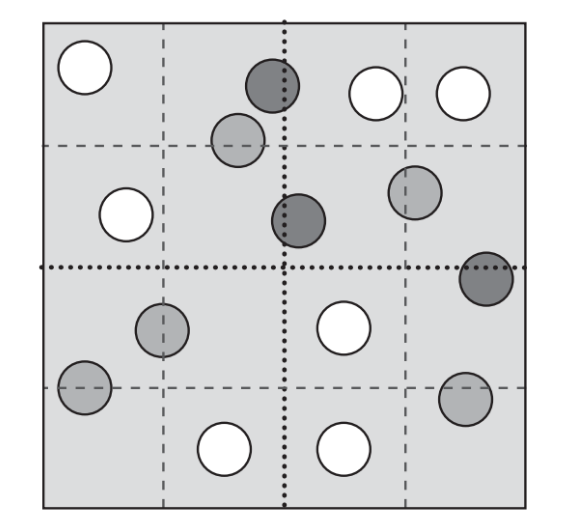
\includegraphics[width=\textwidth]{Imagens/Figura_7.11.png}
	\legend{Fonte: \cite{bourg2013physics}. }
\end{figure}

Descrição da Figura~\ref{fig:figura1}:
A imagem mostra um quadrado com 15 objetos no interior. Os objetos têm forma de circunferência e não há nenhuma colisão entre eles. O quadrado maior (representa o primeiro nível) é então dividido ao meio (na vertical e na horizontal), formando agora 4 subquadrados (representam o segundo nível). Na imagem, esta divisão é feita por linha de pontinhos. A seguir uma nova divisão ocorre e cada subquadrado é dividido novamente (na vertical e na horizontal) em 4 novos subquadrados (representam o terceiro nível). Na imagem, esta divisão é feita por linhas tracejadas. Ao final das divisões, cada quadrado foi dividido em 4 subquadrados (formando na imagem 8 subquadrados)

Os objetos dentro do cubo inicial são agora classificados em função de sua posição estão nesta divisão. Se foram “cortados” por uma das linhas divisórias, então pertencem ao nível superior, caso contrário pertencem ao nível inferior.

A primeira divisão, de linha pontilhada “corta” 3 bolinhas (estão destacadas em cinza escuro). Estas bolinhas pertencem ao cubo inicial (primeiro nível); As linhas tracejadas “cortam” 5 bolinhas (estão destacadas em cinza claro). Estas bolinhas pertencem aos cubos da primeira divisão (segundo nível); As bolinhas que não estão sendo cortadas por nenhuma linha (estão destacadas em branco), ficaram exatamente dentro das divisões menores, pertencendo ao terceiro nível.

\subsubsection{Classificar e Varrer}

Na detecção de colisão, existe uma categoria de algoritmos denominada de
classificação e varredura. Estes algoritmos tem como objetivo determinar grupos
de objetos que estão colidindo uns com os outros. Esta categoria de algoritmos é dividida em duas etapas principais:

Classificação: Classifica os objetos seguindo um critério específico. Este
critério pode ser ordenar os objetos ao longo de um determinado eixo.

Varredura: Varre os objetos classificados detectando interseções entre os os
objetos que estão na projeção do intervalo especificado.

Segundo \citeonline{ericson2004real} o algoritmo começa ordenando o vetor de entrada por um dos eixos X, Y ou Z., em
seguida, o vetor é percorrido, e em cada iteração os objetos são testados
quanto a colisão. Caso o limite inferior do Código~\ref{code:aabb_1} seja maior do
que o limite superior do AABB testado, o laço interno pode parar com segurança
pois não existe mais risco de colisão com os próximos objetos. Em seguida, a
variância dos eixos são calculados, e o eixo com a maior variância é
selecionado para uma execução futura.

\begin{lstlisting}[frame=single,caption=Exemplo de ordenar e varrer\label{code:SortAndSweep}]
void SortAndSweepAABBArray()
{
qsort(gAABBArray, MAX_OBJECTS, sizeof(AABB *), cmpAABBs);
float s[3] = {0.0f, 0.0f, 0.0f}, s2[3] = {0.0f, 0.0f, 0.0f}, v[3];
for (int i = 0; i < MAX_OBJECTS; i++)
{
Point p = 0.5f * (gAABBArray[i]->min + gAABBArray[i]->max);
for (int c = 0; c < 3; c++)
{
s[c] += p[c];
s2[c] += p[c] * p[c];
}
for (int j = i + 1; j < MAX_OBJECTS; j++)
{
if (gAABBArray[j]->min[gSortAxis] > gAABBArray[i]->max[gSortAxis])
break;
if (AABBOverlap(gAABBArray[i], gAABBArray[j]))
TestCollision(gAABBArray[i], gAABBArray[j]);
}
}
for (int c = 0; c < 3; c++)
v[c] = s2[c] - s[c] * s[c] / MAX_OBJECTS;
gSortAxis = 0;
if (v[1] > v[0])
gSortAxis = 1;
if (v[2] > v[gSortAxis])
gSortAxis = 2;
}
\end{lstlisting}

\subsection{Algoritmos de Fase Estreita}

Após  os testes da fase ampla retornarem pares de objetos que possivelmente
estejam colidindo, é a vez da fase estreita ser executada.

Nesta fase, os algoritmos mais custosos e complexos computacionalmente são
executados para determinar com certeza se os objetos estão em colisão.
Caso estejam, pode-se coletar as informações sobre a colisão como normal, ponto
de contato e profundidade de penetração para resolver a colisão mais tarde.

\subsubsection{Esfera contra Esfera}

Para que duas esferas estejam em colisão, a soma de seus raios deve ser menor
ou igual a distância de seus centros segundo \citeonline{ericson2004real}.
A representação da esfera descrita no Código~\ref{code:sphere3d} será utilizada.

\begin{lstlisting}[frame=single,caption=Colisão entre esferas\label{code:collisionSphereSphere}]
bool sphereSphere(sphere3d* s1, sphere3d* s2)
{
vector3d v=s1->center-s2->center;
float dist=((v.x*v.x)+(v.y*v.y)+(v.z*v.z));
float sqRadius=s1->radius+s2->radius;
sqRadius=sqRadius*sqRadius;
if(dist<=sqRadius)
{
return true;
}
return false;
}
\end{lstlisting}

Neste exemplo, a soma dos raios foram elevados ao quadrado para realizar o
teste contra a distância também ao quadrado entre os centros das esferas.
Esta é uma prática recomendada pois o cálculo de raiz quadrada pode ser muito
lento para ser realizada como descrito em \citeonline{ericson2004real} e \citeonline{bourg2013physics}.

\subsubsection{Caixa contra Caixa}

Para que duas caixas estejam em colisão, precisa existir sobreposição nos três
eixos testados.
Neste exemplo, a representação de caixa apresentada no Código~\ref{code:box3d_1} será preferida.

\begin{lstlisting}[frame=single,caption=Colisão entre caixas\label{code:collisionBoxBox}]
bool boxBox(box3d* b1, box3d* b2)
{
if((b1->min.x>b2->max.x)||(b2->min.x>b1->max.x))
return false;
if((b1->min.y>b2->max.y)||(b2->min.y>b1->max.y))
return false;
if((b1->min.z>b2->max.z)||(b2->min.z>b1->max.z))
return false;
return true;
}
\end{lstlisting}

Existem outras variações para este mesmo algoritmo descritos com mais detalhes
em \citeonline{ericson2004real}.

\subsubsection{Esfera contra Caixa}

O teste de esfera e caixa pode ser realizado em duas etapas principais:
Primeiro: encontrar o ponto mais próximo da caixa em relação a esfera.
Segundo: Calcular a distância entre o ponto mais próximo e o centro da esfera.
Caso a distância seja menor que o raio da esfera, então existe uma colisão.

\begin{lstlisting}[frame=single,caption=Colisão entre esfera e caixa\label{code:collisionSphereBox}]
bool spherebox(sphere3d *s, box3d *b)
{
vector3d closestPoint;
for (int i = 0; i < 3; i++)
{
float v = s->center[i];
if (v < b->min[i])
v = b->min[i];
if (v > b->max[i])
v = b->max[i];
closestPoint[i] = v;
}
float sqdist = ((closestPoint - s->center) * (closestPoint - s->center));
float sqradius = (s->radius * s->radius);
if (sqdist <= sqradius)
{
return true;
}
return false;
}
\end{lstlisting}

Implementações mais sofisticadas podem ser encontradas em \citeonline{ericson2004real}.

\subsubsection{Informações sobre a Colisão}

Se o objetivo for determinar  se os objetos colidem, os testes demonstrados são
suficientes. No entanto, se o objetivo for resolver a colisão informações adicionais devem
ser coletadas durante o processo de detecção de colisão. O processo de coleta
de informações é um problema difícil segundo \citeonline{ericson2004real}.
Quais informações coletar depende muito dos objetivos do sistema.

Porém, três informações são fundamentais:
Ponto de contato: Retorna um ou mais pontos de contato indicando onde os objetos colidiram.
Normal da colisão: Este é um vetor unitário apontando a direção em que os objetos devem ser movidos para que eles parem de colidir.
Profundidade de penetração: É o quanto os objetos estão se sobrepondo. Esta
informação é utilizada juntamente com a normal de colisão para calcular o vetor
de translação mínima (VTM) ou (MTV) em inglês, necessário para separar os dois
objetos.

Cuidados Adicionais devem ser tomados ao se determinar a normal da colisão como
por exemplo, se uma esfera colidir contra uma caixa, e seu centro estiver
dentro da caixa, o vetor normal será um vetor nulo, o que poderá resultar em
comportamentos indesejados na hora de resolver a colisão.

\subsection{Resolução de Colisão}

Após detectar uma colisão entre dois objetos torna-se necessário resolver
a mesma. Em simulações que não requerem um realismo muito grande, apenas a
correção das posições dos objetos torna-se necessária.

Em simulações mais avançadas, como simulações de física, outros métodos podem
ser utilizados como a resolução de colisão por impulso.
Neste método, características físicas dos objetos são levados em consideração
para que os objetos reajam de forma adequada e mais natural.

Outro cuidado deve-se ser levado em conta nesta etapa.
Os objetos em colisão podem ser um objeto estático e um objeto dinâmico, ou
dois objetos dinâmicos. A colisão não deve ser resolvida caso os dois objetos
em colisão sejam estáticos.
Caso um dos objetos seja dinâmico e o outro estático, a resolução da colisão
deve atuar apenas no objeto dinâmico.
Caso os dois objetos sejam dinâmicos, a resolução deve atuar sobre os dois
objetos em direções opostas.

O Código~\ref{code:solveCollision} exemplifica este processo.

\begin{lstlisting}[frame=single,caption=Exemplo de resolução de colisão\label{code:solveCollision}]
void solveCollision(object* b1, object* b2, vector3d contactPoint,
 vector3d normal, vector3d depth)
{
if(b1->mass<=0.0f)
{
float dir=dotProduct(r2->velocity, normal);
if(dir>0) return;
if(depth>0)
{
vector3d mtv=normal*depth;
b2->Translate(mtv);
}
float j=-(b2->velocity*normal) * (b2->restitution+1)*b2->mass;
vector3d impulse=(j*info.normal);
r1->velocity+=(1 / r1->mass) * impulse;
}
else
{
}
}
\end{lstlisting}

Segundo \citeonline{bourg2013physics} este é apenas um exemplo básico e simplificado. Em simulações complexas muitos Outros atributos devem ser levados em consideração como tensores de inércia, velocidade tangencial, velocidade angular e torque.

\section{Metodologia}

A  proposta de desenvolvimento deste projeto é um programa gráfico que
executará simulações de movimento em ambientes 3d, para analisar os mecanismos de detecção de colisão.

\subsubsection{Recursos preliminares do Simulador}
O simulador desenvolvido deverá implementar algumas leis básicas da física, para que os objetos simulados reajam de forma mais realista, tornando assim, a simulação mais dinâmica. 

O programa será organizado em 3 partes principais: 
Tela principal: Será onde a simulação será desenhada, mostrando ao usuário o andamento da simulação. A tela principal também terá um menu permitindo o controle de diversos aspectos da simulação. 
Configuração do ambiente: Esta tela será responsável por configurar o ambiente de simulação. Propriedades como limites do ambiente, passo de tempo, e se a gravidade deve ou não ser aplicada são exemplos de propriedades configuráveis. Também nesta tela, terá a lista de objetos que poderão ser controlados.
Engine de simulação: Esta parte do programa será subdividida em simulação do movimento e detecção de colisão. 
Simulação do movimento: Esta etapa é responsável pelos cálculos que modelam o movimento dos objetos presentes no ambiente da simulação, utilizando para isto as leis de Newton. No entanto, a única restrição existente é que os objetos estáticos, que representam obstáculos ou a geografia do espaço, não devem ser movimentados.

Detecção de colisão: A detecção de colisão é a etapa responsável por aplicar algoritmos específicos nos objetos a fim de determinar se existe uma sobreposição, ou se a distância entre 2 objetos é inferior a uma determinada tolerância. Esta etapa também é responsável por resolver a colisão caso exista. 

No simulador, o usuário terá a opção de definir as seguintes variáveis de simulação:
limites espaciais cujo os objetos podem percorrer; 
definir obstáculos; 
aplicar a força da gravidade; 
definir o passo de tempo da simulação; 
Os objetos simulados poderão, por meio de um painel, ter os seguintes parâmetros configuráveis: 
\begin{itemize}
\item massa; 
\item posição;
\item velocidade;
\item coeficiente de restituição;
\item forma. 
\end{itemize}

\subsubsection{Modelagem preliminar do simulador}
Nesta cessão, a modelagem preliminar da engine de simulação será discutida apresentando seus principais componentes.

\begin{lstlisting}[frame=single,caption=Exemplo de vetor3d\label{ps:vec3d}]
classe vetor3d
{
eixo_x
eixo_y
eixo_z
magnitude()
normalizar()
inverso()
produto_escalar()
produto_vetorial()
produto_triplo_escalar()
};
\end{lstlisting}

A classe descrita no Código~\ref{ps:vec3d} representará as coordenadas cartesianas tridimensionais no espaço.
Existem três componentes fundamentais:
eixo_X: Representa a distância do ponto em relação a uma origem de referência horizontalmente.
eixo_y: Representa verticalmente a distância do ponto até a origem.
eixo_z: É o eixo perpendicular ao eixo x e eixo y. Utilizado para dar profundidade.

O Código~\ref{ps:vec3d} também tem diversas operações associadas como soma, subtração,
multiplicação e divisão. Também possui métodos específicos como normalização,
magnitude, inverso e seus produtos como produto vetorial e escalar.

\begin{lstlisting}[frame=single,caption=Exemplo de interface de forma geométrica\label{ps:geometricshape}]
classe FormaGeometrica
{
tipo
recuperar_centroide()
calcular_suporte()
transladar(vetor v)
escalar(s)
rotacionar(orientação)
converter_string()
};
\end{lstlisting}

A classe de forma geométrica apresentada no Código~\{ps:geometricshape}]} é uma base para as próximas implementações de
esferas e caixas.
Ela declara padrões que devem ser seguidos pelas classes filhas.

\begin{lstlisting}[frame=single,caption=Exemplo de esfera 3d\label{ps:sphere3d}]
classe esfera estende FormaGeometrica
{
ponto_central
raio
};
\end{lstlisting}

A classe esfera do Código~\ref{ps:sphere3d} tem 2 atributos principais que são:
Ponto_central: É um vetor que representa as coordenadas centrais da esfera.
Raio: Representa o quanto a esfera se estende em todas as direções a partir do
centro.

\begin{lstlisting}[frame=single,caption=Exemplo de caixa\label{ps:box3d}]
classe caixa  estende FormaGeometrica
{
mínimo
arestas
};
\end{lstlisting}

A classe caixa do Código~\ref{ps:box3d} tem duas propriedades que também são importantes:
Mínimo: É um vetor que representa o canto inferior esquerdo da caixa.
Arestas: É o quanto as arestas se estendem nos 3 eixos a partir do canto
inferior esquerdo...

\begin{lstlisting}[frame=single,caption=Exemplo de AABB\label{ps:aabb}]
classe AABB
{
min
max
FormaGeometrica
translação(vetor v)
escala(s)
escala(vetor v)
computar_volume_delimitador()
};
\end{lstlisting}

A classe apresentada no Código~\ref{ps:aabb}  é responsável por representar um volume delimitador para 
envolver completamente uma forma geométrica, seja ela esfera, caixa ou
poliedro.
A classe possui 3 atributos principais:
min: É um vetor representando o canto inferior esquerdo do aabb...
Max: É um vetor representando o canto superior direito do aabb...
FormaGeometrica: É a forma geométrica que o aabb está contendo...
Também possui métodos para redimensionar e transladar o AABB.

\begin{lstlisting}[frame=single,caption=Exemplo de coletor de informações\label{ps:collisioninfo}]
classe colisao_info
{
ponto_de_colisao
normal_da_colisao
profundidade
objeto_1
objeto_2
};
\end{lstlisting}

O Código~\ref{ps:collisioninfo} da classe CollisionInfo é responsável por conter informações sobre a colisão que
foi detectada como ponto de colisão, normal, profundidade, e os objetos
envolvidos na colisão.

\begin{lstlisting}[frame=single,caption=Exemplo de classe estática para colisões\label{ps:collision3d}]
classe colisao
{
esfera_esfera(s1, s2, info)
esfera_caixa(s, c, info)
caixa_caixa(c1, c2, info)
esfera_poliedro(s, p, info)
caixa_poliedro(c, p, info)
poliedro_poliedro(p1, p2, info)
};
\end{lstlisting}

O Código~\ref{ps:collision3d} da classe de colisão irá conter os métodos específicos de colisão entre as
formas geométricas específicas como esferas x esferas, caixas x caixas e
poliedros x poliedros.

\begin{lstlisting}[frame=single,caption=Exemplo de interface de corpo rígido\label{ps:rigidbody}]
classe corpo_rigido_interface
    {
massa
restituição
nome
aabb
posição
    };
\end{lstlisting}

A interface do Código~\ref{ps:rigidbody} define alguns atributos básicos que será necessário ao modelar o
objeto. Se precisarmos de atributos mais específicos, ou se quisermos expandir
nossa simulação futuramente, basta sub-classificarmos esta interface e realizar
as mudanças necessárias.

\begin{lstlisting}[frame=single,caption=Exemplo de fase ampla\label{ps:broadphase}]
classe fase_ampla
{
escanear(lista_de_objetos, lista_de_possiveis_colisões)
};
\end{lstlisting}

A interface do Código~\ref{ps:broadphase} representa o nosso algoritmo de broadphase. Como existem
diversos algoritmos, optou-se de criar uma interface e realizar a implementação
separadamente.
O método scan recebe um vetor de corpos rígidos para verificar, e também uma
lista onde será armazenado informações sobre uma possível colisão...

\begin{lstlisting}[frame=single,caption=Exemplo de fase estreita\label{ps:narrowphase}]
classe fase_estreita
    {
detectar_colisões(lista_de_possiveis_colisões, lista_de_colisões)
    };
\end{lstlisting}

Este Código~\ref{ps:narrowphase} implementa o algoritmo de fase estreita da mesma forma que a interface
de fase ampla. Este algoritmo recebe uma lista de possíveis colisões e sua
tarefa é aplicar os testes de detecção de colisão entre geometrias específicas
e avaliar se de fato, o par testado está colidindo.

\begin{lstlisting}[frame=single,caption=Exemplo de solucionador de colisões\label{ps:collisionsolver}]
classe solucionador_de_colisão
    {
resolver(lista_de_colisões)
resolver_par(objeto_1, objeto_2, info)
    };
\end{lstlisting}

Este Código~\ref{ps:collisionsolver} irá resolver as colisões detectadas. Ele age separando os corpos se
existir sobreposição, e aplicando impulso...

\begin{lstlisting}[frame=single,caption=Exemplo de integrador numérico\label{ps:integrator}]
classe integrador_numérico
{
mover(lista_de_objetos, tempo)
mover_objeto(objeto, tempo)
};
\end{lstlisting}

Este Código~\ref{ps:integrator} implementa o algoritmo que fará os objetos se movimentarem na simulação. Para isso serão utilizadas equações das leis de Newton.

\begin{lstlisting}[frame=single,caption=Exemplo de octree\label{ps:octree}]
classe octree
{
raiz
adicionar_objeto(objeto)
remover_objeto(objeto)
fase_ampla(lista_de_objetos, lista_de_possíveis_colisões)
fase_ampla(objeto, lista_de_possíveis_colisões)
}

O Código~\ref{ps:octree} da octree é utilizada na fase ampla, mas como ela é relativamente cara de
se construir, ela é utilizada em objetos estáticos como obstáculos que representam a geografia do ambiente simulado.
A classe tem 2 métodos de fase ampla. O primeiro, recebe uma lista de todos objetos
que queremos que sejam testados, e a saída é uma lista com todas as colisões
detectadas. O segundo método, recebe um objeto e uma lista de saída de colisões detectadas.

\begin{lstlisting}[frame=single,caption=Exemplo de ambiente de simulação\label{ps:world}]
class ambiente_de_simulação estende AABB
{
tempo_atual
gravidade
lista_de_objetos
fase_ampla
fase_estreita
solucionador_de_colisões
integrador_numérico
octree
adicionar_objeto(objeto)
remover_objeto(objeto)
passo_de_simulação(tempo)
};
\end{lstlisting}

Este Código~\ref{ps:world} é responsável pela simulação do ambiente. Para isso recebe e manipula todos os objetos instanciados pelas classes anteriormente descritas. A classe permite adicionar e remover objetos, e também definir os algoritmos utilizados
para realizar as tarefas.
O método de atualização será chamado sempre que um passo na simulação for avançado.
Ele primeiramente movimentará os objetos, e então fará a fase ampla, fase
estreita, e resolverá as colisões...

\subsubsection{Requisitos do Projeto}

A listagem a seguir apresenta os recursos previstos para o desenvolvimento do projeto.
Todos os  recursos são  de código aberto, ou possuem licenças de uso não comercial.

\begin{itemize}
\item Compilador compatível com c++20 ou superior;
\item Compilador compatível com C2017 ou posterior;
\item Framework wxwidgets para a criação das telas e controles como listas, botões e demais controles…
\item Biblioteca opengl para a renderização gráfica;
\item wxglade para construir a interface gráfica do usuário (GUI)
\item Biblioteca fmod e bass para indicações sonoras;
\end{itemize}

\subsection{Cronograma}

A listagem a seguir, apresenta uma distribuição estimada das tarefas a serem
realizadas de forma quinzenal.

\begin{enumerate}
\item Agosto:
\begin{itemize}
\item primeira quinzena:
\begin{itemize}
\item Configuração do ambiente de desenvolvimento e modelagem das classes do simulador.
\end{itemize}
\item segunda quinzena:
\begin{itemize}
\item Revisão e testes das classes desenvolvidas
\item Registros e documentação parcial para composição do artigo final
\end{itemize}
\end{itemize}
\item Setembro
\begin{itemize}
\item primeira quinzena:
\begin{itemize}
\item Desenvolvimento da janela principal do aplicativo e seus diálogos.
\end{itemize}
\item segunda quinzena:
\begin{itemize}
\item Desenvolvimento da animação gráfica dos objetos
\item Registro sobre o andamento do projeto para a composição do artigo final
\end{itemize}
\end{itemize}
\item Outubro
\begin{itemize}
\item primeira quinzena
\begin{itemize}
\item Refinamento de todo o projeto desenvolvido e realizar a integração dos componentes.
\end{itemize}
\item segunda quinzena
\begin{itemize}
\item Finalização do protótipo para testes e correções de bugs
\item Registro do progresso para a composição do artigo final
\end{itemize}
\end{itemize}
\item Novembro
\begin{itemize}
\item Primeira quinzena:
\begin{itemize}
\item Testes do protótipo
\item Escrita do artigo final
\end{itemize}
\item Segunda quinzena:
\begin{itemize}
\item Término do artigo final
\end{itemize}
\end{itemize}
\item Dezembro
\begin{itemize}
\item primeira quinzena:
\begin{itemize}
\item Finalização e entrega do artigo final
\item Defesa do Trabalho de conclusão de curso
\end{itemize}
\end{enumerate}
